
\section*{Problema P6.32}

\renewcommand*\thesection{6.32}
\numberwithin{equation}{section}

\begin{center}
    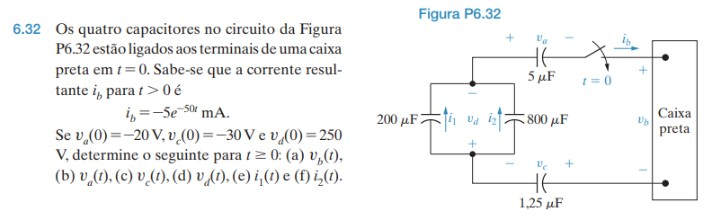
\includegraphics[scale=1.0]{P6.32.jpg}
\end{center}

\subsection*{(a)}

Começamos reduzindo os capacitores a uma capacitância equivalente $C_{eq}$ via redução série-paralelo. 

\[ C_{eq} = (200 \;\mu F \; // \; 800 \;\mu F) + 5 \;\mu F + 1.25 \;\mu F  \]

\[ C_{eq} = 1 \;\mu F  \]

Sabemos que a tensão em um capacitor é dada por

\begin{equation}\label{eq:6.32.1}
    v(t) = v(0) + \frac{1}{C} \int_{t_i}^{t_f} i(t) \,dt
\end{equation}

Usando $i_b(t)$ e a capacitância equivalente, 

\[ v_b(t) = v_b(0) + \frac{1}{C_{eq}} \int_{0}^{t} i_b(t) \,dt \]

Usando análise de malhas em $t=0$, com a corrente de malha $i_b(t)$, podemos identificar $v_b(0)$.

\[ v_b(0) + v_a(0) + v_d(0) + v_c(0) = 0\]

\[ v_b(0) = - (v_a(0) + v_d(0) + v_c(0)) \]

\[ v_b(0) = - (-20 + -30 + 250) \]

\[ v_b(0) = - 200 \un{V} \]

Voltando à \eqref{eq:6.32.1},

\[ v_b(t) = -200 + \frac{1}{1 \;\mu F } \int_{0}^{t} -0.005e^{-50t} \,dt \]

\[ v_b(t) = -200 + 100\left[e^{-50t} - e^0\right] \]

\[ \boxed{v_b(t) = -300 + 100e^{-50t} \un{V}}  \]

\subsection*{(b)}

Ainda usando \eqref{eq:6.32.1}, temos 

\[ v_a(t) = v_a(0) + \frac{1}{C_{a}} \int_{0}^{t} i_b(t) \,dt \]

\[ v_a(t) = -20 + \frac{1}{5 \;\mu F} \int_{0}^{t} -0.005e^{-50t} \,dt \]

\[ v_a(t) = -20 + 20 \left[e^{-50t} - e^0\right] \]

\[ \boxed{v_a(t) = -40 + 20e^{-50t} \un{V}}  \]

\subsection*{(c)}

Ainda usando \eqref{eq:6.32.1}, temos 

\[ v_c(t) = v_c(0) + \frac{1}{C_{c}} \int_{0}^{t} i_b(t) \,dt \]

\[ v_c(t) = -30 + \frac{1}{1.25 \;\mu F} \int_{0}^{t} -0.005e^{-50t} \,dt \]

\[ v_c(t) = -30 + 80 \left[e^{-50t} - e^0\right] \]

\[ \boxed{v_c(t) = 50 + 80e^{-50t} \un{V}}  \]

\subsection*{(d)}

Ainda usando \eqref{eq:6.32.1}, temos 

\[ v_d(t) = v_d(0) + \frac{1}{C_{d}} \int_{0}^{t} i_b(t) \,dt \]

\[ v_d(t) = 250 + \frac{1}{200 \;\mu F + 800 \;\mu F} \int_{0}^{t} -0.005e^{-50t} \,dt \]

\[ v_d(t) = 250 + 0.1 \left[e^{-50t} - e^0\right] \]

\[ \boxed{v_d(t) = 249.9 + 0.1e^{-50t} \un{V}}  \]

\subsection*{(e)}

A corrente em um capacitor é dada por

\begin{equation}\label{eq:6.32.2}
    i(t) = C\diff{v}{t}
\end{equation}

Substituindo,

\[ i_1(t) = (200\;\mu F)(-5e^{-50t}) \]

\[ \boxed{i_1(t) = - e^{-50t} \un{mA}}  \]

\subsection*{(f)}

Novamente usando \eqref{eq:6.32.2}, temos

\[ i_2(t) = (800\;\mu F)(-5e^{-50t}) \]

\[ \boxed{i_2(t) = - 4e^{-50t} \un{mA}}  \]

